\documentclass[10pt,a4paper]{article}
\usepackage[driver=xetex,a4paper,left=45mm,right=45mm,top=30mm,bottom=40mm]{geometry} % propper margins on a4 paper
\usepackage{pdfpages} % to include cover
\usepackage{url}
%\usepackage[hidelinks]{hyperref} % make contents and references clickable in pdf
\usepackage{multicol} % allows multiple colums
\usepackage{titlesec} % adjust whitespace around headings and improves placing
\usepackage{microtype} % adjusts kerning and letterspacing
\usepackage{soul} %striketrough
\usepackage{parskip} % newline instead of indenting
\usepackage{graphicx} % include images
\graphicspath{{graphics/}}

\usepackage{fontspec} % allows custom fonts
\setmainfont[BoldFont=Source Sans Pro Bold,AutoFakeSlant=0.3]{Source Serif Pro}
\setmonofont{Source Code Pro}

\usepackage{listings} % allows code listings
\usepackage{lstautogobble}

\makeatletter
\newcommand\footnoteref[1]{\protected@xdef\@thefnmark{\ref{#1}}\@footnotemark}
\makeatother

\lstdefinelanguage{CSharp}
    {language=[sharp]C,
     morekeywords={var}}

\lstdefinelanguage{FSharp}
    {morekeywords={let, new, match, with, rec, open, module, namespace, type, of, member, and, for, in, do, begin, end, fun, function, try, mutable, if, then, else},
    sensitive=true,
    morecomment=[l][\itshape]{///},
    morecomment=[l][\itshape]{//},
    morecomment=[s][\itshape]{{(*}{*)}},
    morestring=[b]",
    }

\lstdefinelanguage{mc}
    {morekeywords={Func,Data,TypeFunc,Module,TypeAlias,Inherit,is},
     morestring=[b]",
     sensitive=true,
    }

\lstset{basicstyle=\footnotesize\ttfamily,
        breaklines=true,
        keepspaces=true,
        xleftmargin=6pt,
        keywordstyle=\bfseries,
        stringstyle=\itshape,
        %gobble=2, % ignore first 2 spaces indents in code listings
        %frame=single,
        autogobble,
        captionpos=b,
        }

\lstnewenvironment{MC}[1][]{% make code unsplittable
   \noindent
   \minipage{\linewidth} 
   \lstset{language=mc,#1}}
   {\endminipage}

\lstnewenvironment{FS}[1][]{% make code unsplittable
   \noindent
   \minipage{\linewidth} 
   \lstset{language=FSharp,#1}}
   {\endminipage}

\lstnewenvironment{CS}[1][]{% make code unsplittable
   \noindent
   \minipage{\linewidth} 
   \lstset{language=[sharp]C,#1}}
   {\endminipage}

\usepackage[sorting=none,backend=biber]{biblatex} %citations
\addbibresource{references.bib}
\renewcommand*{\bibfont}{\small} % small references at the end

%\usepackage{draftwatermark}
%\SetWatermarkText{DRAFT - DO NOT GRADE}
%\SetWatermarkFontSize{40pt}
%\SetWatermarkLightness{0.8}
%\SetWatermarkAngle{0}
%\SetWatermarkVerCenter{5em}

\begin{document}

% disable page numbers
\pagestyle{empty} 

% cover page
\includepdf[pages=1]{build/cover.pdf}
\newpage

% make subsubsections unnumbered and not show up in the TOC
\setcounter{secnumdepth}{2} 
\setcounter{tocdepth}{2}

% start page numbers
\setcounter{page}{1}
\pagenumbering{arabic}
\pagestyle{plain}

%\begin{multicols}{2}
\tableofcontents
%\columnbreak

\section{Introduction}

\subsection{Working title}
\textit{Design and implementation of the Meta Casanova 3 compiler back-end}

\subsection{Motive}
Kenniscentrum is interested in innovative technologies.
Innovative technologies like virtual reality and video games are the fields our research group is researching.

In order to ease the development of virtual reality and video games, the Casanova language was developed.
The Casanova language is the subject of the PhD thesis of Francesco.

The complex nature of the Casanova language lead to a complex compiler.
To simplify the development of Casanova, the language Meta Casanova was developed.

\subsection{Importance}
The resulting program will be used by the research group to build the meta Casanova 3 compiler, and the resulting thesis will be used as documentation for the future developers of MC.

This will be useful to the research group.

\subsection{Goal}
The goal of the assignment is to have a working back-end that is able to produce an executable.

\subsection{Problem statement}
At the start of the assignment, there is only a definition of MC 2.
At the end of the assignment, there is a working back-end for MC 3.

\subsection{Research question}
The primary research question of this thesis is:

\textit{How to implement a transformation from typechecked Meta Casanova (MC) from the front-end, to executable code within the timeframe of the internship?}

Where the transformation must satisfy these requirements:
\begin{description}
    \item[The correctness requirement] The back-end must in no case produce an incorrect program.
    \item[The .NET requirement] The executable must be able to inter-operate with .NET.
    \item[The multiplatform requirement] The generated code must run on all the platforms .NET runs on.
    \item[The performance requirement] The performance of the generated program should be better than Python.
\end{description}

The correctness requirement exists because the compiler must be reliable.
Any program can at most be as reliable as the compiler used to generate it.
\label{whydotnet}
The .NET requirement exists because of the need for a large library and inter-operability with Unity game engine.
This is because the main area of research of the organization is game-related\footnote{see section~\ref{motive}}.
The multiplatform requirement is because the games are produced for any platform.
The performance requirement is there because games have to be fast.

In order to answer the research question, seven sub-questions were formulated.

\begin{enumerate}
    \item In what language should the code generator produce its output?
    \item What should the interface be between the front-end and the back-end?
    \item What should the intermediate representation of the functions be?
    \item How does the interface map to the output language?
    \item How to generate names so that they comply with the output language?
    \item How to validate the code-generator?
    \item How to validate the test programs?
\end{enumerate}

Each answer of a sub-question is provided evidence by implementing a part of the back-end. 
This will in turn provide evidence to answer the main research question.

\subsection{client}
The graduation assignment is carried out at Kenniscentrum Creating 010.
\textit{Kenniscentrum Creating 010 is a transdisciplinary design-inclusive Research Center enabling citizens, students and creative industry making the future of Rotterdam}~\cite{creating2016home}.

The research group is creating the Casanova language.
The members of the research group are 
  Francesco di Giacomo\footnote{\label{venice}Universita' Ca' Foscari, Venezia}, 
  Mohamed Abbadi\footnoteref{venice}, 
  Agostino Cortesi\footnoteref{venice}, 
  Giuseppe Maggiore\footnote{Hogeschool Rotterdam} and 
  Pieter Spronck\footnote{Tilburg University}.

Within the research group is our research team, tasked with the design and implementation of Meta Casanova.
The research team is supervised by Giuseppe Maggiore and comprises of three students.
Louis van der Burg, responsible for developing the Meta Casanova language,
Jarno Holstein, responsible for the front-end of the Meta Casanova compiler,
and Douwe van Gijn, responsible for the back-end of the Meta Casanova compiler.

\subsection{Workplace and tasks}
During the internship the student will be part of a research team that develops and implements the MC compiler.
The student periodically relay the progress and receive feedback every two weeks.
The student will be supported by the research group.


\section*{Abstract}

\textit{Design and implementation of the Meta Casanova 3 compiler back-end}

\section{method}
\subsection{Research Methods}
I will use a variety of of research methods during the internship.

For the choice of language, I will use a comparitive investigation.
For the other subquestions, I will use a combination of design and experimentation, as I use LEAN prototyping.

\subsection{Information collection}
I will mainly use the internet to find official documentation and to download international standards.
I will also use Google Scholar to find published papers.

\subsection{Validation of findings}
The correctness requirement will be validated by running test programs and comparing the output of the interpreter with the output of the compiler.
The generated code will also be inspected with a debugger to find code generation errors.
Performance requirements will be validated by

\subsection{Validity and reliability of sources}
I will use official documentation and international standards from ECMA International and ISO wherever possible.
The theory is also put in practice, providing evidence that the sources were sound.

\subsection{Project methods}
We will make use of LEAN Rapid Prototyping\cite{lean}.

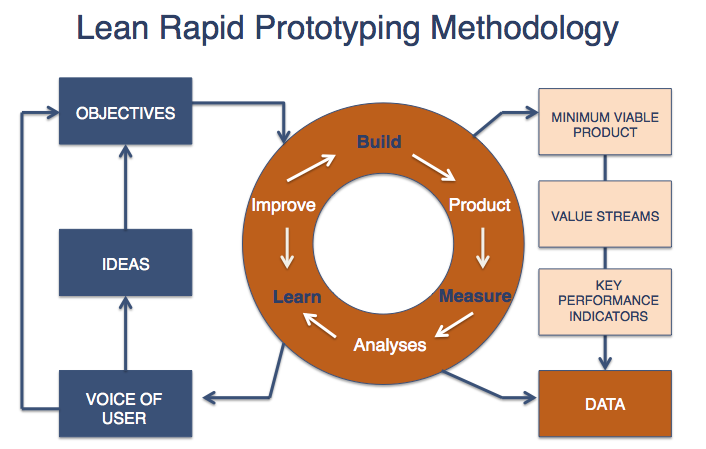
\includegraphics[width=\textwidth]{lean}

This method is great for small teams, as it reduces overhead.
This is crucial because we need to spend our time efficiently if we want to deliver a finished product.
It also allows us to gather knowledge by iterating over our designs.

\subsection{Risk assesment}
\begin{center}
   \begin{tabular}
      {| p{0.2\textwidth} | p{0.28\textwidth} | l | p{0.3\textwidth} |}
      \hline
      \textbf{Risk} & \textbf{Effect} & \textbf{Possibility} & \textbf{Counter measure} \\
      \hline
      No test programs will be available.  & 
	  No emperic mesurements can be done. & 
	  50\% & 
	  I will have to write test programs in the intermediate language \\
	  \hline
      The Type-Checker is not finished in time. &
	  No emperic mesurements on complex programs can't be done. & 
	  50\% & 
	  The complex programs will have to be manually converted to simple programs by me or members of the research-group. \\
      \hline
      The optimisations will not be enough to be faster than python. & 
	  The compiler will not be compettitive with other compilers & 
	  10\% & 
	  Investigate why and report. \\
	  \hline
      Parts are left unfinished due to time constraints. & 
	  Not all requirements will be met & 
	  20\% & 
	  Propper planning an prioritizing low hanging fruit can minimize this. \\
	  \hline
   \end{tabular}
\end{center}

\subsection{Quality expectations}
The quality expectations are encoded in the requirements.


\section{Results}
\subsection{Desired result}

The result will be a working MC compiler that respects the requirements.

\section{Literature}
\subsection{References}
I will use the C\# language standard~\cite{ecma334} and the Common Language Infrastructure(CIL) standard~\cite{ecma335}.
I will also make use of the official .NET compiler documentation on the Microsoft Developer Network~\cite{msdn} as well as the official mono documentation~\cite{mono}.

\printbibliography
%\end{multicols}
\section{Stakeholders}
\begin{tabular} { l l }
    \textbf{Student} & \\
    Name & Douwe van Gijn \\
    Student number & 0864504 \\
    E-mail address & 0864504@hr.nl \\
    Telephone number & +31 6 46 909 730 \\
    & \\
    \textbf{Client} & \\
    Name company & Kennis Centrum Creating 010 \\
    Name company supervisor & Sunil Choenni \\
    E-mail address & h.choenni@hr.nl \\
    Telephone number & +31 6 48 10 03 01  \\
    Function & Lector \\
    Visitors address & Wijnhaven 103 floor 6 \\
    Website company & www.creating010.com \\
    & \\
    \textbf{Company supervisor} & \\
    Name company & Kennis Centrum Creating 010 \\
    Name company supervisor & Sunil Choenni \\
    E-mail address & h.choenni@hr.nl \\
    Telephone number & +31 6 48 10 03 01  \\
    Function & Lector \\
    Visitors address & Wijnhaven 103 floor 6 \\
    Website company & www.creating010.com \\
    & \\
    \textbf{School supervisors} & \\
    Name examinator (first teacher) & Giuseppe Maggiore \\
    E-mail address & +31 6 41 78 12 23 \\
    Telephone number & g.maggiore@hr.nl \\
    & \\
    Name assessor (second teacher) & Hans Manni \\
    E-mail address & j.p.manni@hr.nl \\
    Telephone number & \\
    & \\
    \textbf{School coördinator} & \\
    Name graduate coördinator INF/TI & Aad van Raamt \\
    Telephone number & 010 7944993 \\
    E-mail address & A.van.Raamt@HRO.NL \\
\end{tabular}
\newpage

\end{document}
